{\Large \textbf{\textcolor{Maroon}{Binary choice (1)}}}: \\
\begin{minipage}{0.6\textwidth}
\textbf{Logic program}:
\begin{lstlisting}
num(1).
left(X) :- not right(X), num(X).
right(X) :- not left(X), num(X).
\end{lstlisting}
\end{minipage}
\begin{minipage}{0.4\textwidth}
\textbf{Answer sets}:
\begin{lstlisting}
num(1) left(1)
num(1) right(1)
.
\end{lstlisting}
\end{minipage}

\vspace{0.35cm}

{\Large \textbf{\textcolor{Maroon}{Binary choice (2)}}}: \\
\begin{minipage}{0.6\textwidth}
\textbf{Logic program}:
\begin{lstlisting}
num(1).
num(2).
left(X) :- not right(X), num(X).
right(X) :- not left(X), num(X).
\end{lstlisting}
\end{minipage}
\begin{minipage}{0.4\textwidth}
\textbf{Answer sets}:
\begin{lstlisting}
num(1) num(2) left(1) left(2)
num(1) num(2) right(1) left(2)
num(1) num(2) left(1) right(2)
num(1) num(2) right(1) right(2)
\end{lstlisting}
\end{minipage}

\vspace{0.35cm}

{\Large \textbf{\textcolor{Maroon}{Constraints (1)}}}: \\
\begin{minipage}{0.6\textwidth}
\textbf{Logic program}:
\begin{lstlisting}
num(1).
num(2).
left(X) :- not right(X), num(X).
right(X) :- not left(X), num(X).

:- left(1) $\text{\textcolor{PineGreen}{\# left(1) cannot be true}}$
\end{lstlisting}
\end{minipage}
\begin{minipage}{0.4\textwidth}
\textbf{Answer sets}:
\begin{lstlisting}
num(1) num(2) right(1) left(2)
num(1) num(2) right(1) right(2)


.
\end{lstlisting}
\end{minipage}

\vspace{0.35cm}

{\Large \textbf{\textcolor{Maroon}{Constraints (2)}}}: \\
\begin{minipage}{0.6\textwidth}
\textbf{Logic program}:
\begin{lstlisting}
num(1).
num(2).
left(X) :- not right(X), num(X).
right(X) :- not left(X), num(X).

:- left(1), left(2) $\text{\textcolor{PineGreen}{\# left(1) and left(2) cannot both be true}}$
\end{lstlisting}
\end{minipage}
\begin{minipage}{0.4\textwidth}
\textbf{Answer sets}:
\begin{lstlisting}
num(1) num(2) right(1) left(2)
num(1) num(2) right(1) right(2)
num(1) num(2) left(1) right(2)

.
\end{lstlisting}
\end{minipage}

\vspace{0.35cm}

{\Large \textbf{\textcolor{Maroon}{Constraints vs rules/facts}}} (constraints \textbf{never} add new answer sets): \\
\begin{minipage}{0.6\textwidth}
\textbf{Logic program}:
\begin{lstlisting}
num(1).
num(2).
left(X) :- not right(X), num(X).
right(X) :- not left(X), num(X).

:- not left(1) 
:- not right(1) 
\end{lstlisting}
\end{minipage}
\begin{minipage}{0.4\textwidth}
\textbf{Answer sets}:
\begin{lstlisting}
(none)





.
\end{lstlisting}
\end{minipage}

\vspace{0.35cm}

{\Large \textbf{\textcolor{Maroon}{Constraints vs rules/facts}}} (constraints \textbf{never} add new answer sets): \\
\begin{minipage}{0.5\textwidth}
\textbf{Logic program}:
\begin{lstlisting}
num(1).
num(2).
left(X) :- not right(X), num(X).
right(X) :- not left(X), num(X).

left(1) $\text{\textcolor{PineGreen}{\# now it is a fact}}$
right(1) $\text{\textcolor{PineGreen}{\# now it is a fact}}$
\end{lstlisting}
\end{minipage}
\begin{minipage}{0.5\textwidth}
\textbf{Answer sets}:
\begin{lstlisting}
num(1) num(2) right(1) left(1) right(2)
num(1) num(2) right(1) left(1) left(2)




.
\end{lstlisting}
\end{minipage}

\vspace{0.35cm}


{\Large \textbf{\textcolor{Maroon}{Helpful feature: \# show}}}: \\
\begin{minipage}{0.6\textwidth}
\textbf{Logic program}:
\begin{lstlisting}
num(1).
num(2).
left(X) :- not right(X), num(X).
right(X) :- not left(X), num(X).

:- left(1) 

#show left/1 $\text{\textcolor{PineGreen}{\% format: \# show predicate/arity.}}$
#show right/1
\end{lstlisting}
\end{minipage}
\begin{minipage}{0.4\textwidth}
\textbf{(Projected) answer sets}:
\begin{lstlisting}
right(1) left(2)
right(1) right(2)




.
\end{lstlisting}
\end{minipage}

\vspace{0.5cm}
\textbf{Helpful feature: \# show}: \\
If you want to see a specific part (subset) of the answer set (not changing the problem or answer). \\

\newpage
{\Large \textbf{\textcolor{Maroon}{Abbreviations (1)}}}: \\

\begin{minipage}{0.6\textwidth}
\textbf{Logic program}:
\begin{lstlisting}
num(1..3). $\text{\textcolor{PineGreen}{\#  = num(1). num(2). num(3).}}$
left(X) :- not right(X), num(X).
right(X) :- not left(X), num(X).
:- left(1) 
:- right(2)

#show left/1 
#show right/1
\end{lstlisting}
\end{minipage}
\begin{minipage}{0.4\textwidth}
\textbf{Answer sets}:
\begin{lstlisting}
right(1) left(2) left(3)
right(1) left(2) right(3)




.
\end{lstlisting}
\end{minipage}

\vspace{0.35cm}

{\Large \textbf{\textcolor{Maroon}{Abbreviations (2)}}}: \\

\begin{minipage}{0.6\textwidth}
\textbf{Logic program}:
\begin{lstlisting}
num(a;c). $\text{\textcolor{PineGreen}{\#  = num(a). num(c). }}$
left(X) :- not right(X), num(X).
right(X) :- not left(X), num(X).
:- left(a) 

#show left/1 
#show right/1
\end{lstlisting}
\end{minipage}
\begin{minipage}{0.4\textwidth}
\textbf{Answer sets}:
\begin{lstlisting}
right(a) left(b) 
right(a) right(b) 




.
\end{lstlisting}
\end{minipage}

num(a;c) is equivalent to: num(a). num(c). \textbf{So not up to!} \\

\vspace{0.35cm}

{\Large \textbf{\textcolor{Maroon}{\# const}}}: \\

\begin{minipage}{0.6\textwidth}
\textbf{Logic program}:
\begin{lstlisting}
#const k=2 $\text{\textcolor{PineGreen}{\#  = num(1..2). }}$
num(1..k). 
left(X) :- not right(X), num(X).
right(X) :- not left(X), num(X).
:- left(1) 

#show left/1 
#show right/1
\end{lstlisting}
\end{minipage}
\begin{minipage}{0.4\textwidth}
\textbf{Answer sets}:
\begin{lstlisting}
right(1) left(2) 
right(1) right(2) 




.
\end{lstlisting}
\end{minipage}

\newpage 
{\Large \textbf{\textcolor{Maroon}{ Ternary choice}}}: 

\begin{figure}[ht!]
    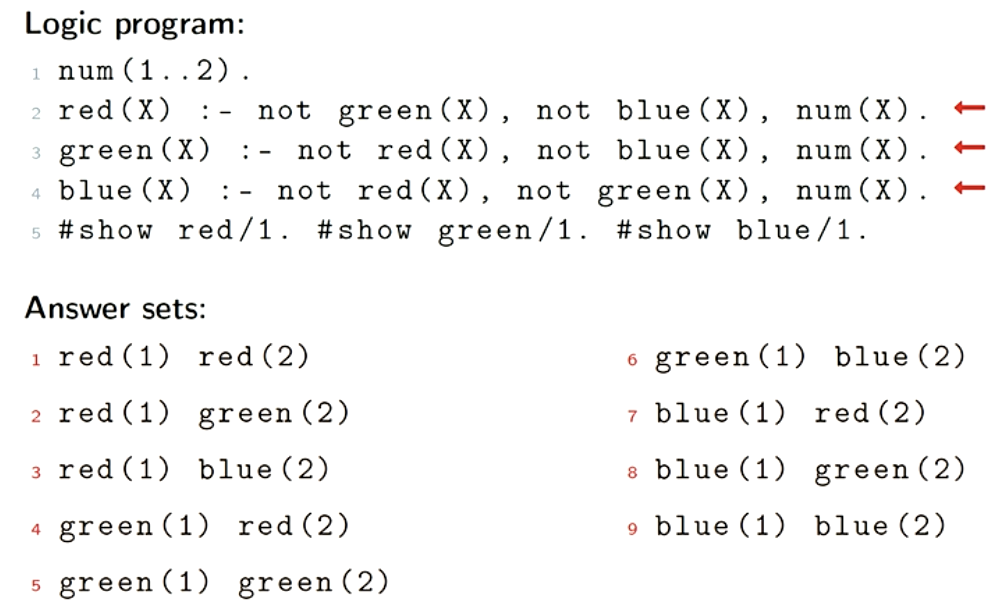
\includegraphics[scale=0.6]{figures/ternary.png}
\end{figure}

\vspace{0.35cm}

{\Large \textbf{\textcolor{Maroon}{Choice rules}}}: \\
\textbf{Logic program}:
\begin{lstlisting}
{ a; b }.
\end{lstlisting}

\begin{minipage}{0.5\textwidth}
Possible translation:
\begin{lstlisting}
a :- not na.
na :- not a.
b :- not nb.
nb :- not b.
\end{lstlisting}
\end{minipage}
\begin{minipage}{0.5\textwidth}
\textbf{Answer sets}:
\begin{lstlisting}
na nb
a nb
na b
a b
\end{lstlisting}
\end{minipage}

\vspace{0.35cm}

\textbf{Choice rule \textcolor{Maroon}{with lower bound}} (choose at least 2 of them): 
\begin{lstlisting}
2 { a; b; c }
\end{lstlisting}
So the anwser set becomes: a b, a c, b c and a b c.\\

\textbf{Choice rule \textcolor{Maroon}{with upper bound}} (choose at most 1 of them): 
\begin{lstlisting}
{ a; b; c } 1
\end{lstlisting}
So the anwser set becomes: \{empty answer set\}, a, and b. \\

\textbf{Choice rule \textcolor{Maroon}{with lower and upper bound}} (choose exactly 2 of them): 
\begin{lstlisting}
2 { a; b; c } 2
\end{lstlisting}
So the anwser set becomes: a b, a c, and b c. \\
\\

{\Large \textbf{\textcolor{Maroon}{Binary choice (1)} - revisited}}: \\
\begin{minipage}{0.7\textwidth}
\textbf{Logic program}:
\begin{lstlisting}
num(1..2).
1 { left(X); right(X) } 1  :- num(X).

.
\end{lstlisting}
\end{minipage}
\begin{minipage}{0.3\textwidth}
\textbf{Answer sets}:
\begin{lstlisting}
left(1) left(2)
right(1) left(2)
left(1) right(2)
right(1) right(2)
\end{lstlisting}
\end{minipage}

\vspace{0.35cm}

{\Large \textbf{\textcolor{Maroon}{Ternary choice} - revisited}}: \\
\begin{minipage}{0.7\textwidth}
\textbf{Logic program}:
\begin{lstlisting}
num(1..2).
1 { red(X); green(X); blue(X) } 1 :- num(X).
#show red/1. 
#show green/1. 
#show blue/1.




.
\end{lstlisting}
\end{minipage}
\begin{minipage}{0.3\textwidth}
\textbf{Answer sets}:
\begin{lstlisting}
red(1) red(2)
red(1) green(2)
red(1) blue(2)
green(1) red(2)
green(1) green(2)
green(1) blue(2)
blue(1) red(2)
blue(1) green(2)
blue(1) blue(2)
\end{lstlisting}
\end{minipage}

\vspace{0.35cm}

{\Large \textbf{\textcolor{Maroon}{Conditional literals (1)}}}: \\
\begin{minipage}{0.6\textwidth}
\textbf{Logic program}:
\begin{lstlisting}
p(1..3).
q(1..2).
s :- p(X) : q(X)
\end{lstlisting}
\end{minipage}
\begin{minipage}{0.3\textwidth}
\textbf{Answer sets}:
\begin{lstlisting}
p(1) p(2) p(3) q(1) q(2) s

.
\end{lstlisting}
\end{minipage}

\vspace{0.35cm}

{\Large \textbf{\textcolor{Maroon}{Conditional literals (2)}}}: \\
\begin{minipage}{0.4\textwidth}
\textbf{Logic program}:
\begin{lstlisting}
p(1..3).
q(1..2).
r(1..3).
s :- p(X) : q(X), r(X)
\end{lstlisting}
\end{minipage}
\begin{minipage}{0.6\textwidth}
\textbf{Answer sets}:
\begin{lstlisting}
p(1) p(2) p(3) q(1) q(2) r(1) r(2) r(3) s


.
\end{lstlisting}
\end{minipage}

\vspace{0.35cm}

{\Large \textbf{\textcolor{Maroon}{Conditional literals (3)}}}: \\
\begin{minipage}{0.4\textwidth}
\textbf{Logic program}:
\begin{lstlisting}
p(1..3).
q(1..2).
r(1..3).
t.
s :- p(X) : q(X), r(X) ; t
\end{lstlisting}
\end{minipage}
\begin{minipage}{0.6\textwidth}
\textbf{Answer sets}:
\begin{lstlisting}
p(1) p(2) p(3) q(1) q(2) r(1) r(2) r(3) s t



.
\end{lstlisting}
\end{minipage}

\vspace{0.35cm}

{\Large \textbf{\textcolor{Maroon}{One-to-one mappings}}}: 
\begin{figure}[ht!]
    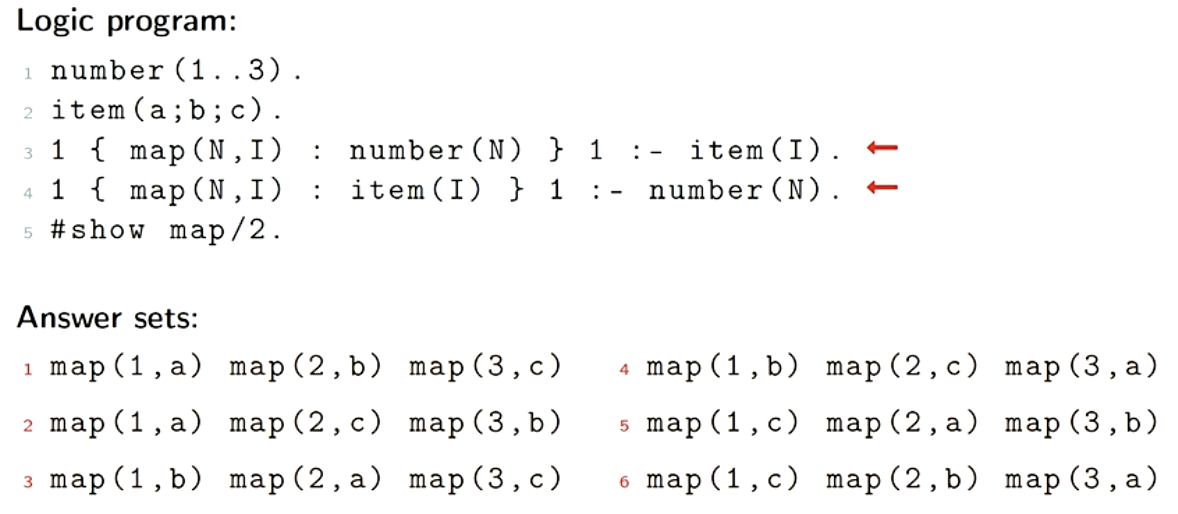
\includegraphics[scale=0.6]{figures/one-to-one.png}
\end{figure}

{\Large \textbf{\textcolor{Maroon}{Computing the sum of some numbers}}}: \\
\textbf{Logic Program}:
\begin{lstlisting}
#const k=4. num(1,5). num(2,2). num(3,6). num(4,2).

sum_so_far(0,0).
sum_so_far(I, OldSum+Num) :- I > 0, I <= k,
    sum_so_far(I-1, OldSum), num(I, Num).
    
sum(M) :- sum_so_far(k, M).
#show sum/1.
\end{lstlisting}

\vspace{0.25cm}

\textbf{Projected answer sets:}
\begin{lstlisting}
sum(15)
\end{lstlisting}

\vspace{0.35cm}

{\Large \textbf{\textcolor{Maroon}{Computing the max of some numbers}}}: 
\begin{lstlisting}
#const k=4. num(1,5). num(2,2). num(3,6). num(4,2).

max_so_far(0,0).
max_so_far(I, Num) :- I > 0, I <= k,
    max_so_far(I-1, OldMax), num(I, Num), num > OldMax.
max_so_far(I, OldMax) :- I > 0, I <= k,
    max_so_far(I-1, OldMax), num(I, Num), Num <= OldMax.
    
max(M) :- max_so_far(k, M).
#show max/1.
\end{lstlisting}

\vspace{0.25cm}

\textbf{Projected answer sets:}
\begin{lstlisting}
max(6)
\end{lstlisting}

\vspace{0.35cm}

{\Large \textbf{\textcolor{Maroon}{More convenient way to sum and max}}}: \\
\textbf{Logic Program}:
\begin{lstlisting}
#const k=4. num(1,5). num(2,2). num(3,6). num(4,2).

sum(S) :- S = #sum { N, num(I,N) : num(I, N) }
max(S) :- M = #max { N, num(I,N) : num(I, N) }

#sum/1. #max/1.
\end{lstlisting}

\vspace{0.25cm}

\textbf{Projected answer sets:}
\begin{lstlisting}
sum(15) max(6)
\end{lstlisting}

\vspace{0.35cm}

{\Large \textbf{\textcolor{Maroon}{Min and count}} (count is unique, other\_count not)}:
\begin{lstlisting}
#const k=4. num(1,5). num(2,2). num(3,6). num(4,2).

min(S) :- S = #min { N, num(I,N) : num(I, N) }
count(S) :- S = #count { N : num(I,N) }
other_count(S) :- S = #count { N, num(I,N) : num(I, N) }


#min/1. #count/1. #other_count/1.
\end{lstlisting}

\vspace{0.25cm}

\textbf{Projected answer sets:}
\begin{lstlisting}
min(2) count(3) other_count(4)
\end{lstlisting}

\vspace{0.35cm}

{\Large \textbf{\textcolor{Maroon}{Computing degree of a graph}}}: \\
Suppose we have an \textcolor{MidnightBlue}{undirected graph $G = (V,E)$}, represented as follows:
\begin{lstlisting}
node(1..5).
edge(1,2). edge(1,3). edge(2,4).
...
edge(X,Y) :- edge(Y,X).
\end{lstlisting}

\begin{itemize}
    \item The \textcolor{Maroon}{degree of a node} in the \textcolor{MidnightBlue}{graph} is the number of nodes that it is connected to.
    \item The \textcolor{Maroon}{degree of the} \textcolor{MidnightBlue}{graph} is the maximum degree of any node in the graph.
\end{itemize}

\textbf{2 ways}: 
\begin{lstlisting}
degree(N, D) :- node(N), D = #count { M : edge(N, M) }
degree(D) :- D = #max { E : degree(N,E), node(N) }
\end{lstlisting}
\textbf{Alternative correct way}: 
\begin{lstlisting}
degree(N, D) :- node(N), D = #count {edge(N,M) : edge(N, M) }
degree(D) :- D = #max { E : degree(N,E) }
\end{lstlisting}

\newpage

\textbf{\textcolor{Maroon}{Warning} on using aggregates}: \\
They are translated by clingo to rules involving regular predicates. The larger the numbers involved, the more rules are needed for the translation, which takes a lot of memory (impacts efficiency of solver). Only use if \textcolor{Maroon}{other constructions provide no solution}.

\subsection*{Optimization}
These statements allow to select between different answer sets. Where we can express what is to be \textcolor{MidnightBlue}{maximized} or \textcolor{MidnightBlue}{minimized}. \textcolor{Maroon}{Optimal answer sets} are those that \textcolor{MidnightBlue}{maximize} or \textcolor{MidnightBlue}{minimize} this criterion.

\begin{lstlisting}
#minimize { N : something(N) }
\end{lstlisting}
expresses that the sum of all N is to be minimized for which something(N) is true (similarly for \#maximize).\\
\\
\textcolor{Maroon}{Be careful}: the part after \#minimize/\#maximize is a \textcolor{Maroon}{set}. So they do not contain duplicates (only counted once). For example:
\begin{lstlisting}
item(1..3).
cost(1,3). cost(2,3). cost(3,2).
2 { choose(I) : item(I) } 2.
#minimize { C,I : choose(I), cost(I,C) }
\end{lstlisting}

\vspace{0.25cm}

\textbf{Projected answer sets:}
\begin{lstlisting}
choose(1) choose(3)
choose(2) choose(3)
\end{lstlisting}

\newpage


{\Large \textbf{\textcolor{Maroon}{Finding all minimum-size dominating sets of an undirected graph G}}}: \\
\\
A \textcolor{Maroon}{dominating set} of an \textcolor{MidnightBlue}{undirected graph $G = (V,E)$} is a subset $D \subseteq V$ of nodes that \textcolor{Maroon}{dominates} all nodes in the graph: for each $v \in V$ either (1) $v \in D$ or (2) $\{u,v\} \in E$ for some $u \in D$. \\
\\
\textbf{Using the 4 steps again} (with an addition of \textcolor{Maroon}{optimization}): 
\begin{enumerate}
    \item \textbf{Formalize the problem}
    \item \textbf{Encoding of problem instances}:
    \begin{enumerate}
        \item State the nodes of the graph using node/1, e.g.:
        \begin{lstlisting}
        node(1..5).
        \end{lstlisting}
        \item State the edges of the graph using edge/2, e.g.:
        \begin{lstlisting}
        edge(1,2). edge(1,3). edge(2,4).
        \end{lstlisting}
        \item State that all edges are also reversed:
        \begin{lstlisting}
        edge(X,Y) :- edge(Y,X).
        \end{lstlisting}
    \end{enumerate}
    \item \textbf{Encoding of candidate solutions (\textcolor{MidnightBlue}{generate}}):
    \begin{enumerate}
        \item Use a choice rule to generate all subsets of nodes, using choose/1:
        \begin{lstlisting}
        { choose(N) : node(N) }.
        \end{lstlisting}
    \end{enumerate}
    \item \textbf{Encoding of solution properties (\textcolor{MidnightBlue}{test}}):
    \begin{enumerate}
        \item Define when a node is \textcolor{PineGreen}{dominated}:
        \begin{lstlisting}
        dominated(N) :- choose(N).
        dominated(N) :- choose(M), edge(N,M).
        \end{lstlisting}
        \item Require that there are  \textcolor{PineGreen}{no undominated} nodes:
        \begin{lstlisting}
        :- node(N), not dominated(N).
        \end{lstlisting}
    \end{enumerate}
    \item \textbf{Add \textcolor{Maroon}{optimization} statements}:
    \item Define when a node is \textcolor{PineGreen}{dominated}:
        \begin{lstlisting}
        #minimize { 1, choose(N) : choose(N) }
        \end{lstlisting}
\end{enumerate}

\newpage

{\Large \textbf{\textcolor{Maroon}{Recursion}}}: \\
\\
Suppose we have an \textcolor{MidnightBlue}{undirected graph $G = (V,E)$}, represented as follows:
\begin{lstlisting}
node(1..5).
edge(1,2). edge(1,3). edge(2,4).
...
edge(X,Y) :- edge(Y,X).
\end{lstlisting}

\vspace{0.35cm}

Always start by having a \textbf{basecase}. Check whether a node is reachable from another, by some path (\textbf{\textcolor{Maroon}{recursively}}):
\begin{lstlisting}
reachable(N,N) :- node(N).
reachable(N,M2) :- reachable(N,M1), edge(M1,M2).
\end{lstlisting}